% !TEX root = ../Ausarbeitung.tex
\section{Learned Approaches}
The next thing we did was trying to learn some of the movements.
We used an evolutionary approach to learn weights for a spiking neural network which controlled the robots movements.

\subsection{Evolutionary Approach}
We first designed a spiking neural network to control the robot.
The network had three input and seven output neurons which were fully connected.
The three dimensional position of the cylinder was used as input.
Six of the output neurons controlled the six joints of the robots arm and the last neuron told the hand when it should release the cylinder.
The individuals of our evolutionary algorithm were vectors with 21 values each representing one weight of the network.
To evaluate the individuals a throw was simulated and the distance of the cylinder from the table represented the fitness of the individual.
After each generation we selected the elite which consists of the best 50\% of the individuals.
The elite was copied into the next generation and the remaining individuals were generated by mutating the individuals of the elite.

\begin{figure}[htbp]
\centerline{\scalebox{.5}{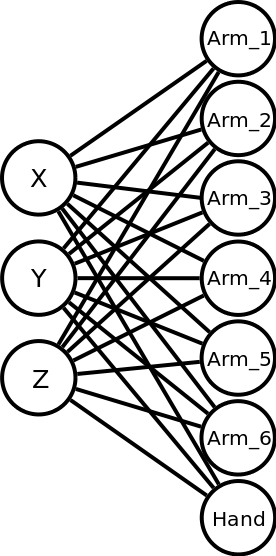
\includegraphics{figures/net.png}}}
\caption{Network architecture.}
\label{fig}
\end{figure}

\subsubsection{Mutation Strategies}
Three different mutation strategies were implemented to generate new descendants.
The first method used only one parent and added or subtracted small random values from its weights.
The other two methods used two parents.
One was a single-point crossover at a random position meaning you take the first n weights from one parent and the remaining ones from the second one.
The last method was a k-point crossover.
At each position this method chose randomly one of the parents weights.

\subsection{Simplified Problem}
As our first learned approach wasn't really successful so we tried to reduce the search space for the evolutionary algorithm.
To achieve this we restricted which joints the robot could use to execute the throw.
We fixed all rotational joints by setting the respective weights in the neural network to zero because we thought this wouldn't impact the robots ability to make a good throw very much.
This reduced the number of weights to be learned from 21 to 12.